\documentclass[12pt,a4paper]{article}
\usepackage{amsmath,amsthm,amssymb,mathtools}
\usepackage{tikz}
\usetikzlibrary{arrows.meta,positioning,shapes.geometric,calc,fit,backgrounds}
\usepackage{graphicx}
\usepackage{booktabs,tabularx,multirow}
\usepackage[ruled,vlined,linesnumbered]{algorithm2e}
\usepackage[most]{tcolorbox}
\usepackage{hyperref}
\usepackage[capitalize,noabbrev]{cleveref}
\usepackage[margin=1in]{geometry}
\usepackage{fancyhdr}
\usepackage{enumitem}
\usepackage{xcolor}

%% ---------------------------------------------------------------
%% tcolorbox environments
%% ---------------------------------------------------------------
\newtcolorbox{keyinsight}[1][]{colback=blue!5!white,colframe=blue!75!black,fonttitle=\bfseries,title=Key Insight,#1}
\newtcolorbox{example}[1][]{colback=green!5!white,colframe=green!75!black,fonttitle=\bfseries,title=Example,#1}
\newtcolorbox{warningbox}[1][]{colback=red!5!white,colframe=red!75!black,fonttitle=\bfseries,title=Warning,#1}

%% ---------------------------------------------------------------
%% amsthm environments
%% ---------------------------------------------------------------
\newtheorem{theorem}{Theorem}[section]
\newtheorem{lemma}[theorem]{Lemma}
\newtheorem{definition}{Definition}[section]
\newtheorem{remark}{Remark}[section]

%% ---------------------------------------------------------------
%% Page style
%% ---------------------------------------------------------------
\pagestyle{fancy}
\fancyhf{}
\rhead{Session 10 -- Deep Feedforward Networks \& Greedy Pre-training}
\lhead{IIIT Dharwad -- Deep Learning}
\cfoot{\thepage}
\renewcommand{\headrulewidth}{0.4pt}

%% ---------------------------------------------------------------
%% Hyperref setup
%% ---------------------------------------------------------------
\hypersetup{
  colorlinks=true,
  linkcolor=blue!60!black,
  citecolor=green!50!black,
  urlcolor=blue!70!black,
  pdftitle={Session 10: Deep Feedforward Networks and Greedy Layer-wise Pre-training},
  pdfauthor={Prof. S R M Prasanna and Dr. Sunil Saumya}
}

%% ---------------------------------------------------------------
%% Convenience macros
%% ---------------------------------------------------------------
\newcommand{\W}{\mathbf{W}}
\newcommand{\x}{\mathbf{x}}
\newcommand{\h}{\mathbf{h}}
\newcommand{\loss}{\mathcal{L}}

\begin{document}

%% ===============================================================
%% TITLE PAGE
%% ===============================================================
\begin{titlepage}
  \centering
  \vspace*{1.5cm}
  {\LARGE\bfseries Deep Learning -- Session 10\par}
  \vspace{0.5cm}
  \rule{\linewidth}{1.5pt}\par
  \vspace{0.4cm}
  {\huge\bfseries Deep Feedforward Networks \&\\[0.3em]
   Greedy Layer-wise Pre-training\par}
  \vspace{0.4cm}
  \rule{\linewidth}{1.5pt}\par
  \vspace{1.2cm}
  {\large\itshape The 2006 Breakthrough: How Deep Networks Became Trainable\par}
  \vspace{1.5cm}
  \begin{tabular}{rl}
    \textbf{Session}      & 10 \\[4pt]
    \textbf{Date}         & December 21, 2025 \\[4pt]
    \textbf{Duration}     & 1 hour 40 minutes \\[4pt]
    \textbf{Instructors}  & Prof.\ S R M Prasanna \\
                          & Dr.\ Sunil Saumya \\[4pt]
    \textbf{Institution}  & Dept.\ of Data Science \& Artificial Intelligence \\
                          & Indian Institute of Information Technology Dharwad \\[4pt]
    \textbf{Slide Deck}   & \texttt{05-PyTorchDL-NNmodule} \\[4pt]
    \textbf{Video}        & \url{https://vimeo.com/1148825885} \\
  \end{tabular}
  \vspace{1.5cm}

  \begin{abstract}
    \noindent
    Session~10 covers the theoretical and empirical foundations of
    \emph{greedy layer-wise pre-training}, the pivotal technique introduced by
    Hinton et al.\ (2006) that made training deep networks feasible for the
    first time.  Starting from the observation that deep networks trained from
    random initialisation performed \emph{worse} than shallow networks due to
    vanishing/exploding gradients, the session explains how treating each hidden
    layer as a Restricted Boltzmann Machine (RBM) and pre-training it in
    isolation provides a principled weight initialisation.  The Bengio et al.\
    (2006, NIPS) supervised variant using auto-encoders is also presented.
    Landmark empirical results are reviewed: the deep generative model achieves
    1.25\% error on MNIST (vs.\ 1.4\% for SVM), and a DBN-DNN with 7 hidden
    layers achieves 17.1\% WER on the HUB500-SWB speech recognition benchmark
    (vs.\ 23.6\% for GMM-HMM).  The session concludes by contextualising why
    greedy pre-training is less necessary today given modern regularisation and
    optimisation advances (ReLU, batch normalisation, Adam), while noting its
    continued relevance for low-resource settings.
  \end{abstract}
\end{titlepage}

%% ===============================================================
%% TABLE OF CONTENTS
%% ===============================================================
\tableofcontents
\newpage

%% ===============================================================
\section{Introduction}
\label{sec:intro}
%% ===============================================================

The history of deep learning is punctuated by a small number of decisive
breakthroughs.  Session~10 focuses on the \textbf{2006 breakthrough} -- the
moment when the research community first demonstrated that deep neural networks
with many layers could be trained reliably and could outperform shallow
alternatives.

Prior to 2006, the neural network field had re-emerged from its first ``AI
winter'' thanks to the backpropagation algorithm, but a new ceiling had been
reached: adding more than two or three hidden layers consistently \emph{failed}
to improve performance, and often made things worse.  The culprits were the
\textbf{vanishing gradient} and \textbf{exploding gradient} problems discussed
in Session~9, which caused gradient-based optimisation starting from random
initialisation to become trapped in poor local minima.

\begin{keyinsight}[title=The Core Problem Before 2006]
  Deep neural networks (DNNs) possess enormous representational capacity,
  being capable of modelling highly non-linear and highly-varying functions.
  Yet in practice, training them from random initialisation using
  backpropagation produced results \emph{worse} than shallow networks with
  one or two hidden layers.  The bottleneck was the optimisation landscape,
  not the model architecture.
\end{keyinsight}

The solution, proposed simultaneously and independently by Hinton et al.\
\cite{hinton2006} and Bengio et al.\ \cite{bengio2006}, was a
\textbf{greedy layer-wise unsupervised pre-training} strategy.  By leveraging
techniques already used in the \emph{feedback} neural network literature
(specifically Restricted Boltzmann Machines) and applying them to
\emph{feedforward} networks, these groups demonstrated that deep networks could
be initialised in a region of weight space from which backpropagation could
refine them effectively.

This session covers:
\begin{enumerate}[leftmargin=*, label=\arabic*.]
  \item Why DNNs failed to train from random initialisation (\cref{sec:background}).
  \item The mechanics of unsupervised greedy layer-wise pre-training (\cref{sec:unsup}).
  \item The Bengio~(2006) supervised variant using auto-encoders (\cref{sec:sup}).
  \item Empirical results on MNIST (\cref{sec:mnist}) and large-vocabulary speech recognition (\cref{sec:asr}).
  \item The legacy and current relevance of pre-training (\cref{sec:legacy}).
\end{enumerate}

\newpage

%% ===============================================================
\section{Background and Prerequisites}
\label{sec:background}
%% ===============================================================

\subsection{Deep Feedforward Networks}

A \emph{deep feedforward network} (DFN), also called a \emph{multilayer
perceptron} (MLP) with many layers, is a directed acyclic graph of parametric
functions.  Given an input vector $\x \in \mathbb{R}^{d_0}$, the network
computes a sequence of hidden representations:

\begin{align}
  \h^{(1)} &= \sigma\!\left(\W^{(1)}\x + \mathbf{b}^{(1)}\right), \label{eq:h1} \\
  \h^{(\ell)} &= \sigma\!\left(\W^{(\ell)}\h^{(\ell-1)} + \mathbf{b}^{(\ell)}\right),
               \quad \ell = 2, \ldots, L, \label{eq:hl} \\
  \hat{y} &= \text{softmax}\!\left(\W^{(L+1)}\h^{(L)} + \mathbf{b}^{(L+1)}\right), \label{eq:yhat}
\end{align}

where $\sigma(\cdot)$ is a pointwise non-linear activation function
(e.g.\ sigmoid or tanh), $\W^{(\ell)}$ and $\mathbf{b}^{(\ell)}$ are the
weight matrix and bias vector for layer $\ell$, and $L$ is the total number
of hidden layers.

\begin{definition}[Depth of a Neural Network]
\label{def:depth}
  The \emph{depth} of a feedforward neural network is the number of
  \emph{hidden} layers $L$.  A network with $L = 1$ is called \emph{shallow};
  a network with $L \geq 2$ is typically called \emph{deep}.
\end{definition}

\subsection{The Vanishing Gradient Problem}

Training by backpropagation requires computing the gradient of the loss
$\loss$ with respect to the weights in every layer.  By the chain rule:

\begin{equation}
  \frac{\partial \loss}{\partial \W^{(1)}} =
  \frac{\partial \loss}{\partial \h^{(L)}} \cdot
  \prod_{\ell=2}^{L} \frac{\partial \h^{(\ell)}}{\partial \h^{(\ell-1)}} \cdot
  \frac{\partial \h^{(1)}}{\partial \W^{(1)}}.
  \label{eq:chain}
\end{equation}

Each Jacobian factor $\partial \h^{(\ell)}/\partial \h^{(\ell-1)}$ has entries
bounded by $\|\W^{(\ell)}\| \cdot \max|\sigma'(\cdot)|$.  For sigmoid
activations, $\max|\sigma'| = 0.25$, so the product in \cref{eq:chain}
\emph{shrinks exponentially} with depth, causing:

\begin{itemize}[leftmargin=*]
  \item \textbf{Vanishing gradients}: $\|\partial \loss / \partial \W^{(1)}\|
        \to 0$; early layers learn extremely slowly or not at all.
  \item \textbf{Exploding gradients}: When weight norms are large,
        the product diverges, causing numerical instability.
\end{itemize}

\begin{warningbox}
  Random weight initialisation places the network in a region of weight space
  where the gradients reaching the early layers are essentially zero.  The
  weights of the first few layers are therefore barely updated during training,
  producing representations no better than random projections of the input.
  This is the fundamental reason deep networks underperformed shallow ones
  before 2006.
\end{warningbox}

\subsection{Why One Hidden Layer ``Was Enough'' -- The Historical Debate}

Interestingly, before 2006, there was a compelling theoretical argument that
one hidden layer \emph{sufficed}:

\begin{theorem}[Universal Approximation, informal]
\label{thm:ua}
  A feedforward network with a single hidden layer of sufficiently many
  neurons can approximate any continuous function on a compact domain to
  arbitrary accuracy.
\end{theorem}

This theorem, combined with empirical results showing that networks with one
large hidden layer matched or exceeded multi-layer networks on tasks such as
speech recognition, led to a working consensus that depth added no benefit.
Support Vector Machines, with their kernel trick (effectively mapping data to
a very high-dimensional space for linear separation), appeared to confirm that
a single nonlinear expansion sufficed.

\begin{remark}
  The universal approximation theorem says \emph{existence} of a solution, not
  that gradient-based optimisation will \emph{find} it.  A single very wide
  layer may require exponentially more neurons than a deep network to represent
  certain functions efficiently.  Depth enables compositional representations
  that shallow networks cannot easily reproduce.
\end{remark}

\subsection{Three Converging Factors Behind the 2006 Breakthrough}

Prof.\ Prasanna emphasised in the lecture that the 2006 breakthrough was not
due to a single invention but to the convergence of three factors:

\begin{enumerate}[leftmargin=*, label=(\roman*)]
  \item \textbf{Large datasets}: The early 2000s saw the large-scale
        collection of labelled data (e.g.\ ImageNet, MNIST, Switchboard
        speech corpus), providing the fuel for data-hungry deep models.
  \item \textbf{GPU computing}: Graphics Processing Units offered
        massively parallel floating-point arithmetic at low cost, making
        large-scale matrix operations feasible.
  \item \textbf{Greedy layer-wise pre-training}: The algorithmic insight
        of Hinton et al.\ (2006) that each layer could be pre-trained
        independently using unsupervised reconstruction provided a principled
        initialisation that escaped poor local minima.
\end{enumerate}

\newpage

%% ===============================================================
\section{Unsupervised Greedy Layer-wise Pre-training}
\label{sec:unsup}
%% ===============================================================

\subsection{The Core Idea}

The term \emph{greedy layer-wise} describes a strategy that breaks an
otherwise intractable joint optimisation problem into a sequence of simpler
sub-problems, each solved independently.  The key observation is:

\begin{keyinsight}[title=Greediness in Pre-training]
  When training a given hidden layer, we \emph{ignore} the effect of all
  higher layers.  We are ``greedy'' in the sense that the sole objective
  for each layer is to best reconstruct its own input.  Since no target
  output is available, this is an \emph{unsupervised} procedure.
\end{keyinsight}

Concretely, consider a DFN with $L = 5$ hidden layers
$H_1, H_2, \ldots, H_5$ between the input $\x$ and the output $\hat{y}$.
Instead of training all weights jointly (which leads to vanishing gradients
at $H_1$), we train one layer at a time:

\begin{enumerate}[leftmargin=*, label=\textbf{Step \arabic*:}]
  \item \textbf{Pre-train $H_1$}: Treat the pair (input layer, $H_1$) as a
        two-layer \emph{feedback} (recurrent) network.  Apply input $\x$,
        propagate forward to $H_1$, then propagate \emph{back} to produce a
        reconstruction $\hat{\x}$.  Minimise the reconstruction error
        $\|\x - \hat{\x}\|^2$.  The resulting weight matrix $\W^{(1)}$
        captures the distribution of $\x$.
  \item \textbf{Pre-train $H_2$}: Pass all training inputs through the
        now-frozen $\W^{(1)}$ to obtain the activations of $H_1$.  Use
        these as the input to a new two-layer feedback network and pre-train
        $\W^{(2)}$ in the same way.
  \item \textbf{Repeat} for $H_3, H_4, H_5$ using the outputs of the
        previously trained layers as inputs.
  \item \textbf{Stack and fine-tune}: Assemble all pre-trained layers into the
        full deep network.  Attach a classification output layer with randomly
        initialised weights $\W^{(L+1)}$.  Fine-tune the entire network
        end-to-end using standard backpropagation (typically for only a few
        epochs, since the weights are already in a good region).
\end{enumerate}

\subsection{Mathematical Formulation of Pre-training a Single Layer}

For layer $\ell$, let the input be $\mathbf{v} \in \mathbb{R}^{d_{\ell-1}}$
(the output of the previous layer, or the raw input for $\ell = 1$).  The
reconstruction objective is:

\begin{equation}
  \min_{\W^{(\ell)}, \mathbf{b}^{(\ell)}}
  \; \mathbb{E}_{\mathbf{v}}\!\left[
    \left\| \mathbf{v} - \hat{\mathbf{v}} \right\|^2
  \right],
  \label{eq:recon}
\end{equation}

where the reconstructed input $\hat{\mathbf{v}}$ is obtained by:

\begin{align}
  \h &= \sigma\!\left(\W^{(\ell)}\mathbf{v} + \mathbf{b}^{(\ell)}\right),
       \label{eq:enc} \\
  \hat{\mathbf{v}} &= \sigma\!\left({\W^{(\ell)}}^{\!\top}\h + \tilde{\mathbf{b}}^{(\ell)}\right).
       \label{eq:dec}
\end{align}

Here ${\W^{(\ell)}}^{\!\top}$ is the transposed weight matrix (tied weights),
acting as the decoder.  Once the reconstruction error is minimised, $\W^{(\ell)}$
encodes a faithful representation of the input data distribution.

\begin{remark}
  The use of tied weights (decoder = encoder$^\top$) in \cref{eq:dec} is not
  mandatory.  In practice, the Hinton group used Restricted Boltzmann Machines
  (RBMs), which learn the weight matrix through contrastive divergence.  For
  the first (visible) layer they used a \emph{Gaussian} RBM (GRBM) to handle
  continuous-valued inputs.  The key distinction between an RBM-based approach
  and a simple auto-encoder is the probabilistic treatment of the hidden
  activations, but conceptually both achieve the same goal: learning a weight
  matrix that preserves the input statistics.
\end{remark}

\subsection{The Role of the Final (Output-Side) Weight Matrix}

A subtle but important point raised in the lecture is why $\W^{(L+1)}$
(the weights connecting the last hidden layer to the output) is \emph{not}
pre-trained and is instead randomly initialised:

\begin{keyinsight}[title=Why $\W^{(L+1)}$ is Randomly Initialised]
  The purpose of pre-training is to provide good generative representations of
  the input.  The output weight matrix $\W^{(L+1)}$ is a \emph{discriminative}
  layer: its job is to separate classes, not to reconstruct the input.
  Because the output layer is directly adjacent to the loss, its gradient is
  large and well-defined during fine-tuning.  There is no vanishing gradient
  problem for $\W^{(L+1)}$; backpropagation can learn it effectively from
  scratch.
\end{keyinsight}

\subsection{The GRBM $\rightarrow$ RBM $\rightarrow$ DBN $\rightarrow$ DBN-DNN Pipeline}

\cref{fig:dbn-pipeline} illustrates the four-step pipeline used by Hinton
et al.\ (2012) for acoustic modelling with DNNs.

\begin{figure}[ht]
\centering
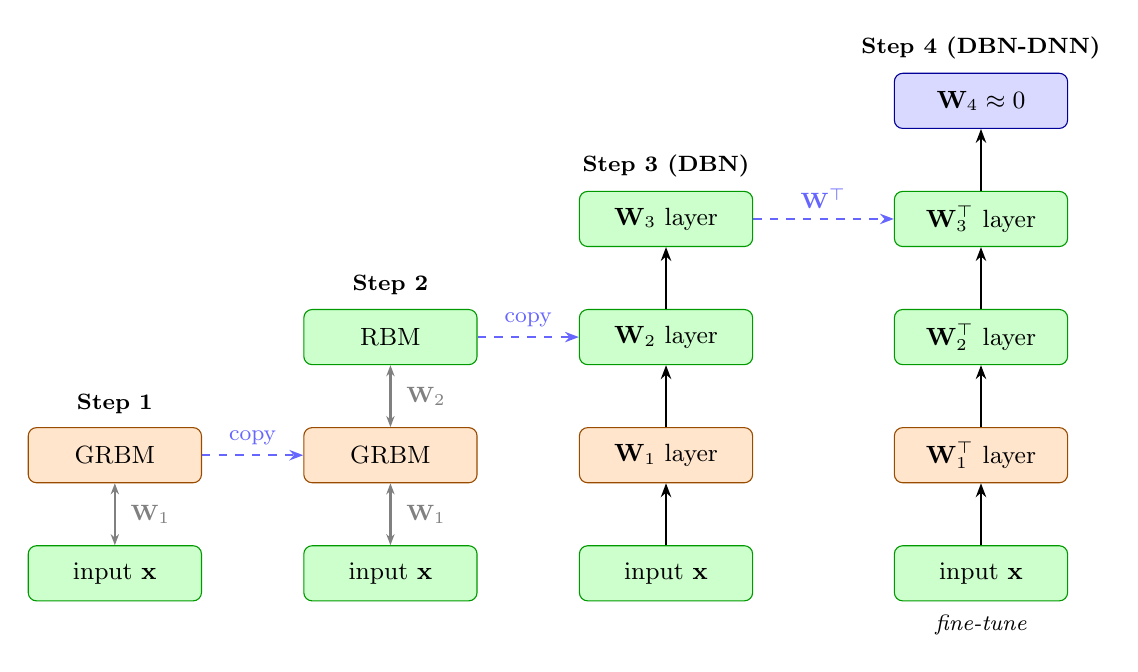
\begin{tikzpicture}[
  every node/.style={font=\small},
  layer/.style={draw, rounded corners=3pt, minimum width=2.2cm, minimum height=0.7cm,
                fill=green!20, draw=green!60!black},
  weight/.style={font=\footnotesize\itshape, midway, right=2pt},
  arr/.style={-{Stealth[length=5pt]}, thick},
  darr/.style={{Stealth[length=4pt]}-{Stealth[length=4pt]}, thick, gray},
  box/.style={draw=gray!70, dashed, rounded corners=5pt, inner sep=6pt}
]

%% Step 1: Train GRBM
\node[layer, fill=orange!20, draw=orange!60!black] (grbm) at (0,1.5) {GRBM};
\node[layer] (in1) at (0,0) {input $\mathbf{x}$};
\draw[darr] (in1.north) -- node[weight]{$\W_1$} (grbm.south);
\node[above=0.05cm of grbm, font=\footnotesize\bfseries] {Step 1};

%% Step 2: Stack RBMs
\node[layer] (rbm2) at (3.5,3.0) {RBM};
\node[layer, fill=orange!20, draw=orange!60!black] (grbm2) at (3.5,1.5) {GRBM};
\node[layer] (in2) at (3.5,0) {input $\mathbf{x}$};
\draw[darr] (in2.north) -- node[weight]{$\W_1$} (grbm2.south);
\draw[darr] (grbm2.north) -- node[weight]{$\W_2$} (rbm2.south);
\node[above=0.05cm of rbm2, font=\footnotesize\bfseries] {Step 2};
\draw[arr, dashed, blue!60] (grbm.east) -- node[above, font=\footnotesize]{copy} (grbm2.west);

%% Step 3: DBN
\node[layer] (w3) at (7,4.5) {$\W_3$ layer};
\node[layer] (w2) at (7,3.0) {$\W_2$ layer};
\node[layer, fill=orange!20, draw=orange!60!black] (w1) at (7,1.5) {$\W_1$ layer};
\node[layer] (in3) at (7,0) {input $\mathbf{x}$};
\draw[arr] (in3.north) -- (w1.south);
\draw[arr] (w1.north) -- (w2.south);
\draw[arr] (w2.north) -- (w3.south);
\node[above=0.05cm of w3, font=\footnotesize\bfseries] {Step 3 (DBN)};

%% Step 4: DBN-DNN fine-tune
\node[layer, fill=blue!15, draw=blue!60!black] (w4) at (11,6.0) {$\W_4 \approx 0$};
\node[layer] (w3t) at (11,4.5) {$\W_3^\top$ layer};
\node[layer] (w2t) at (11,3.0) {$\W_2^\top$ layer};
\node[layer, fill=orange!20, draw=orange!60!black] (w1t) at (11,1.5) {$\W_1^\top$ layer};
\node[layer] (in4) at (11,0) {input $\mathbf{x}$};
\draw[arr] (in4.north) -- (w1t.south);
\draw[arr] (w1t.north) -- (w2t.south);
\draw[arr] (w2t.north) -- (w3t.south);
\draw[arr] (w3t.north) -- (w4.south);
\node[above=0.05cm of w4, font=\footnotesize\bfseries] {Step 4 (DBN-DNN)};
\node[below=0.05cm of in4, font=\footnotesize\itshape] {fine-tune};

%% Arrows between steps
\draw[arr, dashed, blue!60] (rbm2.east) -- node[above, font=\footnotesize]{copy} (w2.west);
\draw[arr, dashed, blue!60] (w3.east) -- node[above, font=\footnotesize]{$\W^\top$} (w3t.west);

\end{tikzpicture}
\caption{The four-step greedy layer-wise pre-training pipeline for
acoustic modelling (Hinton et al., IEEE Signal Processing Magazine, 2012).
GRBM: Gaussian Restricted Boltzmann Machine (used for the visible layer with
continuous inputs); RBM: Restricted Boltzmann Machine for higher layers;
DBN: Deep Belief Network formed by stacking RBMs; DBN-DNN: the DBN weights
are used as initialisation for a discriminatively fine-tuned DNN.
$\W_4 \approx 0$ indicates the output layer is randomly (near-zero) initialised.}
\label{fig:dbn-pipeline}
\end{figure}

\subsection{Why the Term ``Greedy''?}

The term \emph{greedy} has a precise meaning here.  In combinatorial
optimisation, a greedy algorithm makes the locally optimal choice at each
step without considering the global impact.  In the context of layer-wise
pre-training:

\begin{itemize}[leftmargin=*]
  \item When training layer $\ell$, we do not consider layers $\ell+1, \ldots, L$.
  \item The optimisation objective for layer $\ell$ is purely local: minimise
        the reconstruction error of its own input.
  \item Interaction between layers is handled only during the final
        end-to-end fine-tuning phase.
\end{itemize}

This local, independent training sidesteps the vanishing gradient problem
entirely during the pre-training phase, since each sub-network has only two
layers and gradients flow freely.

\newpage

%% ===============================================================
\section{Supervised Greedy Layer-wise Pre-training (Bengio et al., 2006)}
\label{sec:sup}
%% ===============================================================

\subsection{Motivation: Adding Supervision to Pre-training}

Hinton et al.\ (2006) used purely \emph{unsupervised} pre-training -- no
class labels were used during the layer-by-layer initialisation phase.
Bengio et al.\ (2006), published at NIPS~2006, independently confirmed these
results and additionally proposed a \emph{supervised} variant, where each
layer is trained with access to target class information.

\subsection{Auto-encoders as the Supervised Pre-training Vehicle}

The mechanism for supervised pre-training is based on the
\textbf{auto-encoder} architecture.

\begin{definition}[Auto-encoder]
\label{def:autoencoder}
  An \emph{auto-encoder} is a feedforward neural network trained to reproduce
  its input at its output.  Given input $\x$, the network minimises:
  \begin{equation}
    \loss_{\text{AE}} = \|\x - f_{\text{dec}}(f_{\text{enc}}(\x))\|^2,
    \label{eq:ae-loss}
  \end{equation}
  where $f_{\text{enc}}$ is the \emph{encoder} (maps $\x$ to a latent
  representation $\mathbf{z}$) and $f_{\text{dec}}$ maps $\mathbf{z}$ back
  to the input space.  The target output is identical to the input: the
  network is forced to ``look at itself in the mirror.''
\end{definition}

\begin{example}[Auto-encoder for Pre-training Layer 1]
  Suppose the input dimension is 784 (a flattened $28 \times 28$ MNIST image)
  and the first hidden layer has 500 neurons.  For supervised pre-training:
  \begin{enumerate}
    \item Build a three-layer auto-encoder: $784 \to 500 \to 784$.
    \item Set the target output equal to the input.
    \item Train with MSE loss until convergence.
    \item Discard the decoder ($784$-dimensional output layer) and the weight
          matrix connecting $H_1$ to the decoder.
    \item Retain the \emph{encoder} weights $\W^{(1)}$ as the pre-trained
          initialisation for the first hidden layer of the full DNN.
  \end{enumerate}
\end{example}

\subsection{Algorithm: Supervised Greedy Layer-wise Training}

\cref{alg:supervised-glw} formalises the Bengio et al.\ supervised pre-training
procedure.

\begin{algorithm}[H]
\caption{Supervised Greedy Layer-wise Pre-training (Bengio et al., 2006)}
\label{alg:supervised-glw}
\SetAlgoLined
\DontPrintSemicolon
\KwIn{Training set $\{(\x_i, y_i)\}_{i=1}^{N}$; number of hidden layers $L$;
      hidden layer sizes $d_1, d_2, \ldots, d_L$}
\KwOut{Pre-trained weight matrices $\W^{(1)}, \W^{(2)}, \ldots, \W^{(L)}$}
\BlankLine
\tcp{Phase 1: Layer-by-layer pre-training}
Let $\mathbf{V}^{(0)} \leftarrow \{\x_i\}_{i=1}^{N}$ \tcp*{raw inputs}
\For{$\ell \leftarrow 1$ \KwTo $L$}{
  Build a 1-hidden-layer auto-encoder network:
  $\mathbf{V}^{(\ell-1)} \xrightarrow{\W^{(\ell)}} H_\ell \xrightarrow{{\W^{(\ell)}}^\top} \hat{\mathbf{V}}^{(\ell-1)}$\;
  Train using SGD to minimise $\loss_\ell = \|\mathbf{V}^{(\ell-1)} - \hat{\mathbf{V}}^{(\ell-1)}\|^2$\;
  \textbf{Discard} the decoder weights ${\W^{(\ell)}}^\top$\;
  Propagate: $\mathbf{V}^{(\ell)} \leftarrow \sigma(\W^{(\ell)}\mathbf{V}^{(\ell-1)} + \mathbf{b}^{(\ell)})$
  \tcp*{outputs of $H_\ell$ become inputs for $H_{\ell+1}$}
}
\BlankLine
\tcp{Phase 2: Fine-tuning}
Assemble full DNN: $\x \to H_1 \to H_2 \to \cdots \to H_L \to \hat{y}$\;
Add logistic regression output layer with random weights $\W^{(L+1)}$\;
Fine-tune entire network end-to-end with SGD minimising cross-entropy:
\begin{equation*}
  \loss_{\text{CE}} = -\frac{1}{N}\sum_{i=1}^{N} \log p(y_i \mid \x_i; \W^{(1)}, \ldots, \W^{(L+1)})
\end{equation*}
\KwRet{$\W^{(1)}, \ldots, \W^{(L+1)}$}
\end{algorithm}

\subsection{Key Differences Between Unsupervised and Supervised Variants}

\cref{tab:unsup-vs-sup} summarises the key differences between the two
approaches.

\begin{table}[ht]
\centering
\caption{Comparison of unsupervised (Hinton 2006) and supervised (Bengio 2006)
greedy layer-wise pre-training.}
\label{tab:unsup-vs-sup}
\begin{tabularx}{\linewidth}{lXX}
\toprule
\textbf{Aspect} & \textbf{Unsupervised (Hinton 2006)} & \textbf{Supervised (Bengio 2006)} \\
\midrule
Pre-training mechanism & Restricted Boltzmann Machine (RBM / GRBM); contrastive divergence & Auto-encoder; standard SGD with MSE loss \\[4pt]
Use of labels & No labels during pre-training & No labels during pre-training; labels used only in fine-tuning \\[4pt]
Reconstruction target & Hidden-to-visible reconstruction via $\W^\top$ & Output layer reconstructs input ($\hat{\x} = \x$) \\[4pt]
MNIST test error & \textbf{1.25\%} & 1.4\% \\[4pt]
Conceptual clarity & Probabilistic generative model & Deterministic encoder-decoder \\[4pt]
Fine-tuning & Backpropagation (few epochs) & SGD on cross-entropy (full fine-tuning) \\
\bottomrule
\end{tabularx}
\end{table}

\begin{keyinsight}[title=Unsupervised Pre-training is Superior to Supervised]
  The MNIST results in \cref{tab:unsup-vs-sup} reveal that the unsupervised
  RBM-based approach (1.25\%) outperforms the supervised auto-encoder approach
  (1.4\%).  Bengio et al.\ argued that this is because unsupervised
  pre-training captures the full data distribution, including structure that
  may not be directly predictive but still provides a better parameter space
  region for fine-tuning.  The supervised auto-encoder pre-training, while
  better than random initialisation, does not capture the generative structure
  as richly.
\end{keyinsight}

\newpage

%% ===============================================================
\section{Empirical Results: MNIST Handwritten Digit Recognition}
\label{sec:mnist}
%% ===============================================================

\subsection{The MNIST Dataset}

The Modified National Institute of Standards and Technology (MNIST) dataset
consists of $28 \times 28$ grey-scale images of handwritten digits 0--9.
The standard benchmark split comprises 60,000 training images and 10,000 test
images.  Each image is flattened to a 784-dimensional vector for input to a
fully-connected network.

By the mid-2000s, MNIST was considered a nearly-solved problem, with SVMs
achieving 1.4\% error.  Any improvement of $\geq 0.1\%$ at this performance
level was considered statistically significant because the absolute error rate
was already so low.

\subsection{Network Architecture}

The Hinton et al.\ (2006) generative model uses the architecture:

\begin{equation}
  \underbrace{784}_{\text{input}} \to
  \underbrace{500}_{H_1} \to
  \underbrace{500}_{H_2} \to
  \underbrace{2000}_{H_3} \to
  \underbrace{10}_{\text{output}},
  \label{eq:mnist-arch}
\end{equation}

with weight matrices $\W^{(1)} \in \mathbb{R}^{500 \times 784}$,
$\W^{(2)} \in \mathbb{R}^{500 \times 500}$,
$\W^{(3)} \in \mathbb{R}^{2000 \times 500}$, and
$\W^{(4)} \in \mathbb{R}^{10 \times 2000}$.

The pre-training procedure trains $\W^{(1)}, \W^{(2)}, \W^{(3)}$ using the
greedy layer-wise RBM approach.  $\W^{(4)}$ is randomly initialised and
trained only during fine-tuning via backpropagation.

\subsection{Results}

\cref{tab:mnist-results} reproduces the comparison table from the lecture
slides.

\begin{table}[ht]
\centering
\caption{MNIST digit recognition error rates (test set).
         A change of 0.1\% is statistically significant at this performance level.}
\label{tab:mnist-results}
\begin{tabular}{lc}
\toprule
\textbf{Model} & \textbf{Test Error (\%)} \\
\midrule
\textbf{Proposed generative model (784-500-500-2000-10)} & \textbf{1.25} \\
Support Vector Machine (SVM) & 1.40 \\
Backprop (784-500-300-10, cross-entropy + weight decay) & 1.51 \\
Backprop (784-800-10, cross-entropy + early stopping) & 1.53 \\
Backprop (784-500-15-10, squared-error + online updates) & 2.95 \\
\bottomrule
\end{tabular}
\end{table}

\begin{example}[Reading the MNIST Results Table]
  The five rows in \cref{tab:mnist-results} represent a spectrum of
  approaches:
  \begin{itemize}
    \item Row~1 is the deep generative model with greedy pre-training.
          Its 1.25\% error beats the SVM benchmark by 0.15\%
          (more than 0.1\%, hence statistically significant).
    \item Row~2 is the classical machine learning champion (SVM) -- a
          non-neural, kernel-based method at 1.4\%.
    \item Rows~3--5 show standard backpropagation DNNs trained from
          random initialisation.  They are \emph{all worse} than the SVM,
          confirming the problem: without pre-training, deep networks fail.
    \item The worst result (2.95\%) comes from a network with a bottleneck
          hidden layer of only 15 neurons, illustrating that insufficient
          capacity in intermediate layers degrades performance sharply.
  \end{itemize}
\end{example}

\subsection{Effect of Hidden Layer Width}

Bengio et al.\ (2006) also conducted an experiment varying the number of
neurons in the hidden layers closest to the output (specifically replacing the
2000-neuron layer with fewer neurons).  Results showed that decreasing the
width caused monotonically increasing error rates, indicating that:

\begin{itemize}[leftmargin=*]
  \item Large intermediate representations are necessary.
  \item Shallow networks that perform well on training data (near-zero training
        error) often generalise poorly, indicating overfitting rather than
        genuine learning of the data manifold.
  \item The brittleness of shallow networks (error rising steeply as capacity
        is reduced) contrasts with the robustness of deep networks with
        pre-training.
\end{itemize}

\newpage

%% ===============================================================
\section{Empirical Results: DNN for Acoustic Modelling in Speech Recognition}
\label{sec:asr}
%% ===============================================================

\subsection{Background: ASR and the GMM-HMM Baseline}

Automatic Speech Recognition (ASR) systems map a sequence of acoustic feature
vectors to a word sequence.  The classical architecture is:

\begin{itemize}[leftmargin=*]
  \item \textbf{Acoustic model}: A Continuous-Density Hidden Markov Model
        (CD-HMM) with Gaussian Mixture Model (GMM) emission distributions,
        trained on phoneme-labelled speech frames.
  \item \textbf{Language model}: An $n$-gram model over word sequences.
  \item \textbf{Decoder}: A Viterbi or beam-search decoder combining
        acoustic and language model scores.
\end{itemize}

The standard evaluation metric is the \textbf{Word Error Rate (WER)}, defined
as:

\begin{equation}
  \text{WER} = \frac{S + D + I}{N} \times 100\%,
  \label{eq:wer}
\end{equation}

where $S$, $D$, $I$ are the number of substitutions, deletions, and insertions
respectively in the recognised transcript relative to the reference, and $N$ is
the total number of words in the reference.

Before 2012, the state-of-the-art GMM-HMM system on the HUB500-SWB (Switchboard)
benchmark achieved approximately 23.6\% WER, a figure that had remained
essentially static for nearly a decade despite significant engineering effort.

\subsection{The DBN-DNN Architecture for ASR}

Hinton et al.\ (2012) replaced the GMM emission model in the HMM with a
DNN trained using greedy layer-wise pre-training:

\begin{enumerate}[leftmargin=*, label=\arabic*.]
  \item \textbf{Feature extraction}: Mel Frequency Cepstral Coefficients
        (MFCCs) or filter-bank energies from speech frames, typically with
        context windows ($\pm 5$ neighbouring frames) to capture temporal
        dynamics.
  \item \textbf{DBN pre-training}: A stacked GRBM (for the visible layer
        with continuous inputs) followed by binary RBMs for higher layers,
        trained greedily.
  \item \textbf{DNN fine-tuning}: The pre-trained DBN is used to initialise
        a DNN, which is then fine-tuned discriminatively with cross-entropy
        loss to classify phoneme states.
  \item \textbf{HMM integration}: The DNN provides posterior probabilities
        $P(\text{state} \mid \text{features})$, which replace the GMM
        emission scores in the HMM decoder.
\end{enumerate}

\subsection{TikZ Diagram: DBN-DNN ASR Pipeline}

\begin{figure}[ht]
\centering
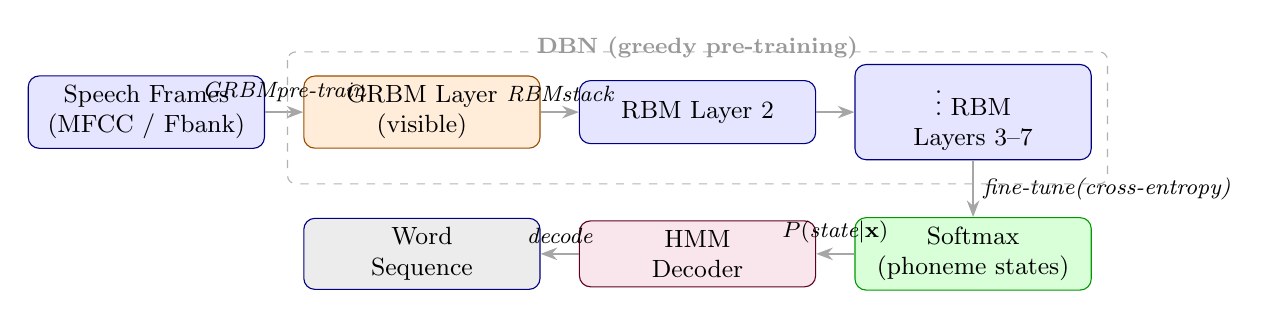
\begin{tikzpicture}[
  every node/.style={font=\small},
  block/.style={draw, rounded corners=4pt, minimum width=3.0cm, minimum height=0.8cm,
                align=center, fill=blue!10, draw=blue!50!black},
  arrow/.style={-{Stealth[length=6pt]}, thick, draw=gray!70},
  label/.style={font=\footnotesize\itshape}
]
\node[block] (feat) at (0,0) {Speech Frames\\(MFCC / Fbank)};
\node[block, fill=orange!15, draw=orange!60!black] (grbm) at (3.5,0) {GRBM Layer\\(visible)};
\node[block] (rbm1) at (7,0) {RBM Layer 2};
\node[block] (rbm2) at (10.5,0) {$\vdots$ RBM\\Layers 3--7};
\node[block, fill=green!15, draw=green!60!black] (softmax) at (10.5,-1.8) {Softmax\\(phoneme states)};
\node[block, fill=purple!10, draw=purple!50!black] (hmm) at (7,-1.8) {HMM\\Decoder};
\node[block, fill=gray!15] (words) at (3.5,-1.8) {Word\\Sequence};

\draw[arrow] (feat.east) -- node[above, label]{GRBM\\pre-train} (grbm.west);
\draw[arrow] (grbm.east) -- node[above, label]{RBM\\stack} (rbm1.west);
\draw[arrow] (rbm1.east) -- (rbm2.west);
\draw[arrow] (rbm2.south) -- node[right, label]{fine-tune\\(cross-entropy)} (softmax.north);
\draw[arrow] (softmax.west) -- node[above, label]{$P(\text{state}|\mathbf{x})$} (hmm.east);
\draw[arrow] (hmm.west) -- node[above, label]{decode} (words.east);

\draw[dashed, gray!60, rounded corners=3pt]
  ($(grbm.north west)+(-0.2,0.3)$) rectangle ($(rbm2.south east)+(0.2,-0.3)$);
\node[above, font=\footnotesize\bfseries, gray!80] at (7, 0.55) {DBN (greedy pre-training)};
\end{tikzpicture}
\caption{End-to-end pipeline for DBN-DNN acoustic modelling in ASR.
The DBN (dashed box) is pre-trained greedily layer-by-layer; the full system
is then fine-tuned discriminatively and integrated into an HMM decoder.}
\label{fig:asr-pipeline}
\end{figure}

\subsection{WER Comparison Results}

\cref{tab:wer-results} reproduces the landmark WER comparison table from the
lecture slides (Hinton et al., IEEE Signal Processing Magazine, Nov.\ 2012).

\begin{table}[ht]
\centering
\caption{Word Error Rate (\%) for various acoustic modelling techniques on the
HUB500-SWB and RT03S-FSH benchmarks (Hinton et al., 2012).
\#Params is in millions; NZ = non-zero parameters after sparsification.}
\label{tab:wer-results}
\begin{tabular}{lccc}
\toprule
\textbf{Modelling Technique} & \textbf{\#Params ($\times 10^6$)} &
\textbf{HUB500-SWB WER\%} & \textbf{RT03S-FSH WER\%} \\
\midrule
GMM, 40 mix DT 309H SI & 29.4 & 23.6 & 27.4 \\
NN 1 hidden layer $\times$ 4,634 units & 43.6 & 26.0 & 29.4 \\
+ 2$\times$5 neighbouring frames & 45.1 & 22.4 & 25.7 \\
\textbf{DBN-DNN 7 hidden $\times$ 2,048 units} & \textbf{45.1} & \textbf{17.1} & \textbf{19.6} \\
+ updated state alignment & 45.1 & 16.4 & 18.6 \\
+ sparsification & 15.2 (NZ) & 16.1 & 18.5 \\
\midrule
GMM 72 mix DT 2000H SA & 102.4 & 17.1 & 18.6 \\
\bottomrule
\end{tabular}
\end{table}

\begin{keyinsight}[title=The Speech Recognition Breakthrough]
  The DBN-DNN with 7 hidden layers $\times$ 2,048 units achieves \textbf{17.1\%}
  WER on HUB500-SWB -- a \textbf{6.5 percentage point} absolute improvement
  over the GMM baseline (23.6\%) and a staggering \textbf{8.9 point}
  improvement over a standard 1-hidden-layer NN (26.0\%).
  Four major research groups (Microsoft, Google, IBM, and the Hinton group)
  independently confirmed similar results around the same time, which gave the
  community high confidence that deep learning was a genuine breakthrough for
  speech recognition.
  For context, the speech recognition community had been struggling to reduce
  error rates below the 27\% range for nearly 30 years.
\end{keyinsight}

\subsection{Significance of the Speech Results}

Several aspects of \cref{tab:wer-results} deserve careful interpretation:

\begin{enumerate}[leftmargin=*, label=\arabic*.]
  \item \textbf{1-hidden-layer NN fails}: The single-hidden-layer NN (26.0\%)
        is actually \emph{worse} than the GMM (23.6\%), even with neighbouring
        frames.  This confirms that raw neural networks without proper
        initialisation cannot compete with well-tuned classical models.
  \item \textbf{Depth matters}: Adding more context frames (22.4\%) helps,
        but the 7-layer DBN-DNN (17.1\%) achieves a qualitatively different
        level of performance.
  \item \textbf{Comparable to a much larger GMM}: The DBN-DNN with 45.1M
        parameters matches the 102.4M-parameter GMM trained on \emph{six
        times more data} (2000 hours vs.\ 309 hours).  This is a dramatic
        demonstration of the data efficiency of deep representations.
  \item \textbf{Sparsification}: Pruning the network to 15.2M non-zero
        parameters (sparsification) barely degrades performance, indicating
        that the network has learnt a compact, distributed representation.
\end{enumerate}

\newpage

%% ===============================================================
\section{The Legacy of Greedy Pre-training and Modern Alternatives}
\label{sec:legacy}
%% ===============================================================

\subsection{Why Pre-training Is Less Necessary Today}

A student question in the lecture prompted Prof.\ Prasanna to address the
contemporary relevance of greedy pre-training.  Since 2012, several advances
have largely superseded the need for layer-wise pre-training when large amounts
of data are available:

\begin{enumerate}[leftmargin=*, label=(\roman*)]
  \item \textbf{ReLU activations}: The Rectified Linear Unit,
        $\sigma(z) = \max(0, z)$, has a gradient of 1 for positive inputs,
        which dramatically reduces the severity of the vanishing gradient
        problem compared to sigmoid/tanh.
  \item \textbf{Batch Normalisation}: Normalising layer inputs during
        training smooths the loss landscape, enabling reliable training of
        very deep networks from random initialisation.
  \item \textbf{Residual connections}: Skip connections in ResNets provide
        identity paths for gradients, allowing networks hundreds of layers
        deep to be trained directly.
  \item \textbf{Advanced optimisers}: Adam, RMSProp, and other adaptive
        learning-rate methods navigate the optimisation landscape more
        effectively than vanilla SGD.
  \item \textbf{Large datasets and transfer learning}: With millions of
        labelled training examples, models can be trained from scratch
        efficiently; and pre-trained models (e.g.\ BERT, GPT) provide
        powerful generic representations that can be fine-tuned.
\end{enumerate}

\begin{table}[ht]
\centering
\caption{Comparison of training regimes: greedy pre-training (2006) vs.\ modern
end-to-end training.}
\label{tab:modern-vs-pretrain}
\begin{tabular}{lcc}
\toprule
\textbf{Aspect} & \textbf{Greedy Pre-training (2006)} & \textbf{Modern End-to-end} \\
\midrule
Activation function & Sigmoid / tanh & ReLU / GELU \\
Weight initialisation & Layer-by-layer RBM/AE & Xavier / He initialisation \\
Normalisation & None & Batch norm, Layer norm \\
Gradient flow & Poor (vanishing) & Stable (residuals, ReLU) \\
Data requirement & Small to medium & Medium to large \\
Training complexity & High (two phases) & Single phase \\
Still useful? & Low-resource settings & General use \\
\bottomrule
\end{tabular}
\end{table}

\subsection{When Pre-training Still Matters}

As Prof.\ Prasanna explicitly noted: \emph{``if you have less amount of data,
for example you have a few hours of data and you want to train the deep
learning model, this greedy layer-wise training is still useful.''}

The modern analogue of greedy pre-training is \textbf{transfer learning} --
the practice of initialising a model with weights pre-trained on a large
dataset (e.g.\ ImageNet, Common Crawl) before fine-tuning on a target task.
This preserves the spirit of the 2006 insight: starting in a good region of
weight space reduces the burden on the final discriminative fine-tuning step.

\begin{keyinsight}[title=The Enduring Principle]
  The fundamental insight of Hinton and Bengio (2006) was not merely an
  engineering trick: it demonstrated that \emph{good weight initialisation
  matters enormously} for deep network training.  Modern techniques
  (He initialisation, batch normalisation, residual connections) achieve the
  same goal -- placing the initial weights in a region where gradient flow is
  healthy -- by different means.  Greedy pre-training solved the right
  problem; later advances solved it more efficiently.
\end{keyinsight}

\subsection{Connection to Modern Self-supervised Learning}

There is a deep conceptual connection between 2006-era greedy unsupervised
pre-training and modern self-supervised learning methods:

\begin{itemize}[leftmargin=*]
  \item \textbf{BERT} (Devlin et al., 2019) pre-trains a Transformer by
        masking and reconstructing tokens -- a form of auto-encoding at the
        sequence level.
  \item \textbf{Contrastive learning} (SimCLR, MoCo) pre-trains visual
        encoders by learning representations invariant to augmentations.
  \item \textbf{wav2vec~2.0} pre-trains speech encoders by discretising and
        reconstructing speech features -- directly analogous to the acoustic
        modelling pipeline in \cref{sec:asr}.
\end{itemize}

In all these cases, unsupervised/self-supervised pre-training provides a
better initialisation than random weights, and the model is then fine-tuned
discriminatively -- precisely the two-phase strategy of Hinton et al.\ (2006).

\newpage

%% ===============================================================
\section{Session Summary and Conclusions}
\label{sec:summary}
%% ===============================================================

Session~10 presented the theoretical foundations and landmark empirical
evidence for the 2006 breakthrough in deep learning.  The following key
points summarise the session:

\begin{enumerate}[leftmargin=*, label=\textbf{\arabic*.}]
  \item \textbf{The problem}: Deep networks trained from random initialisation
        suffered from vanishing/exploding gradients, performing no better --
        and often worse -- than shallow networks or SVMs (e.g.\ 2.95\% MNIST
        error vs.\ 1.4\% SVM).

  \item \textbf{The insight}: The greedy layer-wise algorithm, previously used
        in the \emph{feedback} (RBM) network literature, could be repurposed
        for initialising \emph{feedforward} deep networks.

  \item \textbf{The unsupervised variant} (Hinton et al., 2006): Pre-train
        each layer as a GRBM/RBM using reconstruction error as the objective.
        Stack the pre-trained layers to form a Deep Belief Network (DBN), then
        fine-tune end-to-end.  Result: \textbf{1.25\%} MNIST error (vs.\
        1.4\% SVM).

  \item \textbf{The supervised variant} (Bengio et al., 2006, NIPS): Pre-train
        each layer as a 1-hidden-layer auto-encoder with the input as its own
        target.  Discard the decoder.  Fine-tune end-to-end.  Result:
        comparable to SVM; weaker than unsupervised, but proved the concept.

  \item \textbf{Speech recognition breakthrough}: Four major groups
        (Microsoft, Google, IBM, Hinton) independently demonstrated that
        DBN-DNN acoustic models reduced WER from 23.6\% to 17.1\% on
        HUB500-SWB -- a 6.5 point absolute improvement after decades of
        stagnation around 27\%.

  \item \textbf{Historical significance}: These two papers -- Hinton (2006)
        and Bengio (2006) -- are the cornerstone papers of the modern deep
        learning era.  They provided the algorithmic proof-of-concept that
        directly motivated the investment and research that produced AlexNet
        (2012), Transformers (2017), and large language models.

  \item \textbf{Modern relevance}: Greedy pre-training is no longer the
        standard method for large-data regimes, superseded by ReLU, batch
        normalisation, residual connections, and Adam.  However, for
        low-resource settings, its principles remain valid and are echoed
        in modern self-supervised and transfer learning approaches.
\end{enumerate}

\begin{example}[Timeline of Breakthroughs Covered in Sessions 1--10]
  \begin{center}
  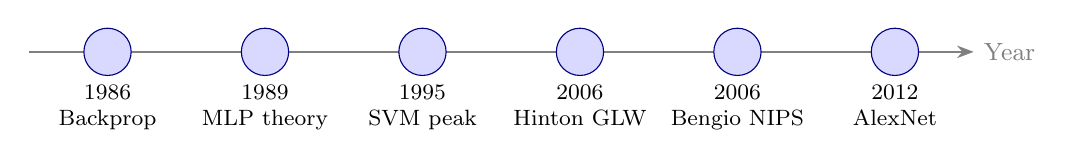
\begin{tikzpicture}[
    every node/.style={font=\small},
    event/.style={circle, draw=blue!50!black, fill=blue!15, minimum size=0.6cm},
    timeline/.style={-{Stealth[length=6pt]}, thick, gray}
  ]
  \draw[timeline] (0,0) -- (12,0) node[right]{Year};
  \foreach \x/\yr/\lab in {
    1/1986/Backprop,
    3/1989/MLP theory,
    5/1995/SVM peak,
    7/2006/Hinton GLW,
    9/2006/Bengio NIPS,
    11/2012/AlexNet/DNN ASR
  }{
    \node[event] at (\x,0) {};
    \node[below=0.3cm, align=center, font=\footnotesize] at (\x,0) {\yr\\\lab};
  }
  \end{tikzpicture}
  \end{center}
\end{example}

\subsection{Take-away Messages}

\begin{itemize}[leftmargin=*]
  \item \textbf{Conceptual}: A good initialisation is as important as the
        architecture.  Greedy pre-training solved initialisation; modern
        techniques (He init, BN, residuals) solve it differently.
  \item \textbf{Practical}: When data is scarce, consider layer-wise
        pre-training or transfer learning before end-to-end training.
  \item \textbf{Historical}: Read the Hinton 2006 and Bengio 2006 papers.
        As Prof.\ Prasanna noted, ``there is no mathematical equation
        there'' -- great ideas are often elegant and simple.
  \item \textbf{Forward-looking}: The self-supervised learning paradigm
        (BERT, wav2vec, CLIP) is the modern embodiment of the same core
        principle: pre-train on reconstruction/contrastive objectives, then
        fine-tune discriminatively.
\end{itemize}

\newpage

%% ===============================================================
\section*{References}
\addcontentsline{toc}{section}{References}
%% ===============================================================

\begin{enumerate}[leftmargin=*, label={[\arabic*]}]

  \item G.\ E.\ Hinton, S.\ Osindero, and Y.-W.\ Teh, ``A fast learning
        algorithm for deep belief nets,'' \textit{Neural Computation},
        vol.\ 18, no.\ 7, pp.\ 1527--1554, 2006.

  \item Y.\ Bengio, P.\ Lamblin, D.\ Popovici, and H.\ Larochelle,
        ``Greedy layer-wise training of deep networks,''
        \textit{Advances in Neural Information Processing Systems (NIPS)},
        vol.\ 19, 2006.

  \item G.\ E.\ Hinton, L.\ Deng, D.\ Yu, G.\ Dahl, A.\ Mohamed,
        N.\ Jaitly, A.\ Senior, V.\ Vanhoucke, P.\ Nguyen, T.\ N.\ Sainath,
        and B.\ Kingsbury,
        ``Deep neural networks for acoustic modeling in speech recognition,''
        \textit{IEEE Signal Processing Magazine}, vol.\ 29, no.\ 6,
        pp.\ 82--97, Nov.\ 2012.

  \item G.\ Tesauro, ``Practical issues in temporal difference learning,''
        \textit{Machine Learning}, vol.\ 8, no.\ 3--4, pp.\ 257--277, 1992.

  \item I.\ Goodfellow, Y.\ Bengio, and A.\ Courville,
        \textit{Deep Learning}. MIT Press, 2016.
        \url{https://www.deeplearningbook.org}

  \item Y.\ LeCun, L.\ Bottou, Y.\ Bengio, and P.\ Haffner,
        ``Gradient-based learning applied to document recognition,''
        \textit{Proceedings of the IEEE}, vol.\ 86, no.\ 11,
        pp.\ 2278--2324, 1998.

  \item J.\ Devlin, M.-W.\ Chang, K.\ Lee, and K.\ Toutanova,
        ``BERT: Pre-training of deep bidirectional transformers for
        language understanding,'' \textit{NAACL-HLT}, 2019.

\end{enumerate}

\vspace{2em}
\hrule
\vspace{0.5em}
\noindent\small\textit{These notes were compiled from the lecture transcript
and visual extractions of Session~10 (Video: \url{https://vimeo.com/1148825885};
Slides: \url{https://learning.iiitdwd.ac.in/mod/resource/view.php?id=1352}).
Department of Data Science and Artificial Intelligence,
Indian Institute of Information Technology Dharwad.}

\end{document}
